\chapter{Results}

\section{Overview}

The developed system integrates Facial Emotion Recognition (FER) and sentiment analysis to interpret user emotions, with both modalities working independently but optimised for their respective domains. The FER system combines face detection and emotion classification, both optimised to enhance accuracy and efficiency. For face detection,  Tiny YOLO, YOLO, HOG+Linear SVM, and Haar Cascade were evaluated based on performance metrics including precision, speed, and robustness. While Tiny YOLO and YOLO were specifically trained to achieve the capability to detect faces, HOG+Linear SVM and Haar Cascade were utilised directly from their respective libraries, Dlib and OpenCV. A comparative analysis of these models identified the most effective solution for real-time emotion recognition tasks.

The emotion classification component used advanced models, including MobileNetV2, ResNet50, and VGG16, leveraging transfer learning techniques. These pre-trained architectures were fine-tuned using labelled emotion datasets to improve their performance for the specific task. During the development process, data augmentation techniques were applied to the dataset to enhance classification accuracy. A comparative analysis of these models highlighted the balance between computational efficiency and classification accuracy.

The sentiment analysis system, using text-based emotion recognition, utilised the cloud-based IBM Watson platform. Rather than being developed from the ground up, this component was selected for its advanced capabilities and tested to ensure seamless integration with the broader system. ChatGPT, a Large Language Model (LLM), was employed to generate speech via a synthesiser, facilitating conversational interactions between the system and users. This user speech was subsequently analysed by IBM Watson to extract sentiment information. Both components were evaluated for their response times, with IBM Watson additionally assessed for its accuracy in identifying sentiments.

\section{Facial Emotion Detection}

This section explores the facial recognition system utilised in the multimodal emotion recognition framework. It encompasses the detailed training methodologies, performance evaluations, and datasets used in the development of facial detection and emotion classification models. The section provides an in-depth analysis of the integration of various detection algorithms, including Haar cascades, dlib, and YOLO (You Only Look Once), alongside the implementation of CNN architectures MobileNetV2, VGG16, and ResNet50 for emotion detection. The comprehensive overview aims to elucidate the effectiveness and efficiency of the system in recognising and interpreting human emotions from facial expressions.

Considering the constrained computational resources inherent in robotic systems, the approach prioritises efficiency without compromising accuracy in emotion recognition. Robots often operate in resource-constrained environments, where computational overhead must be carefully managed to ensure smooth and efficient functioning. In this robot emotion recognition system, the approach is to balance accuracy and computational efficiency. Initially, the intent is to employ a Haar cascade, dlib's HOG + linear SVM, or the YOLO algorithm to locate the face within the robot's camera feed accurately. The use of these algorithms ensures that the subsequent emotion recognition model receives the expected input of only the facial region.

\begin{figure}[!htb]
    \centering{}
    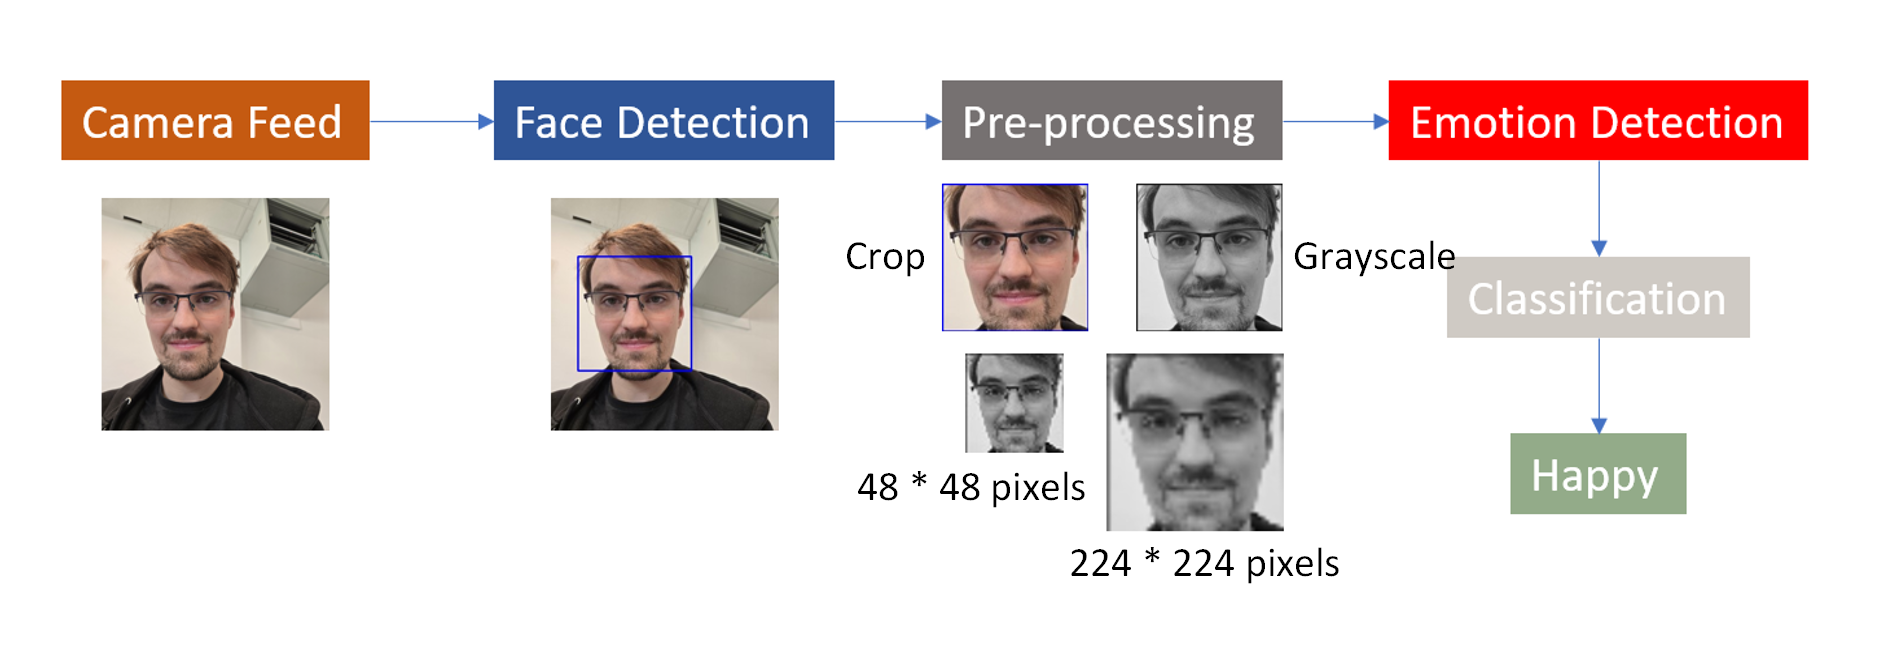
\includegraphics[scale=0.85]{fed_images/pipeline.png}
    \caption{System Pipeline}
    \label{figure:pipeline}
\end{figure}

\subsection{Face Detection}

\subsubsection{Training}

To effectively utilise YOLO, it is necessary to undergo training from scratch or fine-tuning on a specific dataset to suit the intended purpose. This entails collecting a vast dataset of labelled images where each object of interest is annotated with its bounding-box coordinates and class labels.

The models were trained using the recommended YOLOv4 settings from the Darknet GitHub page, by changing the config file which details the training settings: batch size set to 64, subdivisions set to 16, network size width and height both set to 416, and max\_batches set to 6000. Although max\_batches is typically calculated as the number of classes multiplied by 2000, which would result in 2000 for a single class, the minimum allowable value is 6000. Therefore, this value was adjusted accordingly to meet the training requirements.
Each [yolo] layer has a \texttt{classes} parameter, which is set to 80 by default in the cloned repository, as the dataset was originally trained on the COCO dataset. This parameter needs to be adjusted to 1 to match the single class in our dataset. Consequently, the filter settings in the [convolutional] layer preceding each [yolo] layer must also be updated. The number of filters is calculated as:

\[
\text{filters} = (\text{classes} + 5) \times 3
\]

Substituting \(\text{classes} = 1\), the filters are set to:

\[
\text{filters} = (1 + 5) \times 3 = 18
\]

These changes ensure that the model predicts only one class.

Changing the Tiny-YOLO config follows the same process as full YOLO; however, there are only 2 [yolo] layers instead of 3. Lastly, both models have their own pre-trained weights file that was included to assist with training. The final command used in each is shown below.

\noindent{} See the following commands:
\begin{lstlisting}[language=bash]
  $ ./darknet detector train data/obj.data \
        yolov4_face.cfg data/yolov4.conv.137 -map -gpus 0,1
  $ ./darknet detector train data/obj.data \
        yolov4_tiny_face.cfg data/yolov4-tiny.conv.29 \
            -map -gpus 0,1
\end{lstlisting}

\subsubsection{Performance}

To ensure the effectiveness of the YOLO model in detecting faces for subsequent emotion recognition tasks, its performance is evaluated using a variety of metrics. These metrics offer a comprehensive view of the accuracy, speed, and robustness of the model.

In this section, the performance of the YOLO and Tiny YOLO object detection models was evaluated using the WIDER Face dataset, a widely used benchmark for face detection tasks. This dataset contains a diverse range of face images, including variations in scale, pose, occlusion, and illumination, making it an effective testbed for assessing model robustness. To further analyze performance under different conditions, the dataset was split into images containing multiple faces and those containing only one face.

The evaluation employed several key performance metrics: precision, recall, F1 score, average Intersection over Union (IoU), and Average Precision (AP). Precision measures the accuracy of positive predictions, calculated as the ratio of true positives (correctly detected faces) to the sum of true positives and false positives (incorrect detections). High precision indicates that most of the detected faces are actual faces. The inclusion of the WIDER Face dataset ensured a rigorous assessment of the face detection models, highlighting their strengths and weaknesses in varying real-world scenarios.

Precision measures the accuracy of positive predictions. It is calculated as the ratio of true positives (correctly detected faces) to the sum of true positives and false positives (incorrect detections). High precision means that most of the faces detected by the model are actual faces.

\[
\text{Precision} = \frac{\text{True Positives}}{\text{True Positives} + \text{False Positives}}
\]

Recall, or sensitivity, measures the ability of the model to find all relevant instances. It is the ratio of true positives to the sum of true positives and false negatives (missed detections). High recall means that the model can detect most if not all of the faces present in a given image.

\[
\text{Recall} = \frac{\text{True Positives}}{\text{True Positives} + \text{False Negatives}}
\]

The F1 score is the harmonic mean of precision and recall, providing a single metric to evaluate the model's overall performance. It balances the trade-off between precision and recall and is especially useful as an evaluation metric in binary classification.

\[
\text{F1} = 2 \times \frac{\text{Precision} \times \text{Recall}}{\text{Precision} + \text{Recall}}
\]

Intersection over Union measures the overlap between the predicted bounding box and the ground truth bounding box. It is calculated by dividing the overlap area by the union area between the two boxes. A higher IoU means the predicted bounding box closely matches the actual bounding box. An example of the area of overlap can be seen in figure \ref{figure:iou} and the area of union can be seen in \ref{figure:union}.

\begin{figure}[!htb]
    \centering{}
    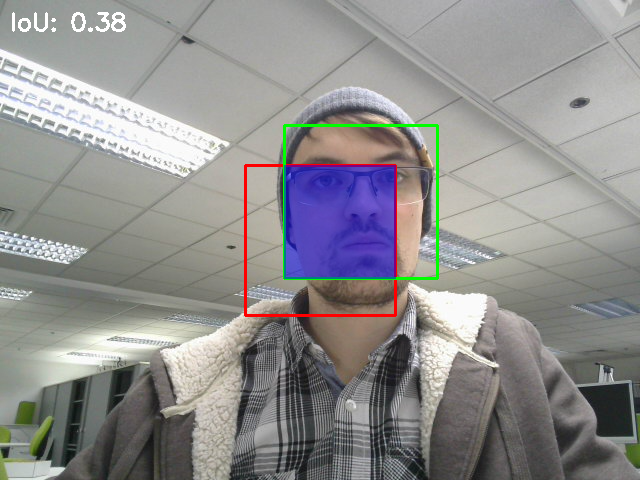
\includegraphics[scale=0.35]{fed_images/iou_overlap.png}
    \caption{An example of IoU, the red box is the predicted bounding box and the green box is the ground truth bounding box. The blue area is the overlap.}
    \label{figure:iou}
\end{figure}

\begin{figure}[!htb]
    \centering{}
    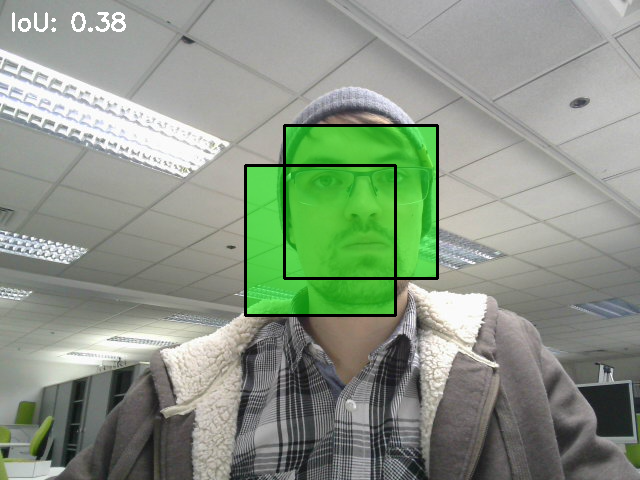
\includegraphics[scale=0.35]{fed_images/iou_individual_boxes.png}
    \caption{The union area of the predicted bounding box and the ground truth bounding box, represented by the total green highlighted area, used in the IoU calculation.}
    \label{figure:union}
\end{figure}

\[
\text{IoU} = \frac{\text{Area of Overlap}}{\text{Area of Union}}
\]

Classification models often output a probability score indicating the likelihood that a given input belongs to a particular class. To make a definitive class prediction, this probability is compared against a predetermined threshold. For instance, in a binary classification scenario, if the threshold is set at 0.5, inputs with a probability above 0.5 are classified as positive, while those below are classified as negative. Adjusting this threshold affects the model's sensitivity (true positive rate) and specificity (true negative rate), allowing practitioners to balance between false positives and false negatives based on the application's requirements.

By varying the confidence threshold and observing the resulting performance, a Receiver Operating Characteristic (ROC) curve can be constructed. This curve plots the true positive rate (sensitivity) against the false positive rate (1-specificity) at different threshold levels. Specificity, or the true negative rate, measures the proportion of actual negatives correctly identified by the model and is calculated as:

\[
\text{Specificity} = \frac{\text{True Negatives (TN)}}{\text{True Negatives (TN)} + \text{False Positives (FP)}}
\]

The area under the ROC curve (AUC) quantifies the model's performance across all thresholds, with a higher AUC indicating better discrimination ability. An AUC of 0.5 suggests no discrimination (random guessing), while an AUC of 1.0 indicates perfect discrimination.

The precision-recall curve is another evaluation metric, particularly useful in scenarios with imbalanced datasets. It plots precision against recall across different threshold values. This curve helps in understanding the trade-off between precision and recall for different threshold settings, providing insights into how well the model balances between identifying positive instances and avoiding false positives.

In the context of face detection models like YOLO and Tiny YOLO, confidence scores are provided with each prediction, enabling the construction of ROC and precision-recall curves by varying the threshold and observing changes in performance metrics. However, models such as Haar Cascade and dlib's HOG+Linear SVM do not output confidence scores with their detections. This absence makes it challenging to adjust thresholds and generate the corresponding curves. Thus neither a precision-recall curve nor an ROC curve can be generated for these models.

Average Precision (AP) is a metric used to evaluate classification models, especially in imbalanced datasets. It summarises the precision-recall curve into a single value, reflecting the model's ability to balance precision and recall across thresholds. AP is calculated by first sorting the predicted scores in descending order, then computing precision and recall at each threshold. Precision measures the proportion of true positives among positive predictions, while recall shows the proportion of true positives among all actual positives.

The area under the precision-recall curve (AUC) represents the AP, which can be calculated as:

\[
\text{AP} = \sum_n (R_n - R_{n-1}) P_n
\]

Where \(P_{n}\) and \(R_{n}\) are the precision and recall at the nth threshold. AP values range from 0 to 1, with higher values indicating better performance. An AP of 1.0 signifies perfect performance, while closer to 0 suggests poor performance. AP provides a comprehensive measure of a model's ability to identify positive instances while minimising false positives.

\begin{table}[h!]
\centering{}
\caption{Performance of YOLO on on the Wider Face dataset and the single face and multi face subsets}
\begin{tabular}{|l|c|c|c|}
\hline
\textbf{Metric}      & \textbf{Wider Face} & \textbf{Multi Face}  & \textbf{Single Face} \\ \hline
\textbf{Precision}   & 0.61        & 0.61            & 0.95                 \\ \hline
\textbf{Recall}      & 0.64        & 0.63            & 0.92                 \\ \hline
\textbf{F1 Score}    & 0.63        & 0.62            & 0.94                 \\ \hline
\textbf{Average IoU} & 45.77\%     & 45.12\%            & 80.90\%              \\ \hline
\textbf{AP}          & 63.17\%     & 62.11\%              & 97.39\%              \\ \hline
\end{tabular}
\label{tab:YOLO}
\end{table}

\begin{table}[h!]
\centering{}
\caption{Performance of Tiny YOLO on the Wider Face dataset and the single face and multi face subsets}
\begin{tabular}{|l|c|c|c|}
\hline
\textbf{Metric}      & \textbf{Wider Face} & \textbf{Multi Face}  & \textbf{Single Face} \\ \hline
\textbf{Precision}   & 0.48        & 0.47            & 0.95                 \\ \hline
\textbf{Recall}      & 0.44        & 0.43            & 0.91                 \\ \hline
\textbf{F1 Score}    & 0.46        & 0.45            & 0.93                 \\ \hline
\textbf{Average IoU} & 35.32\%     & 34.46\%            & 78.08\%              \\ \hline
\textbf{AP}          & 36.63\%     & 35.04\%             & 92.33\%              \\ \hline
\end{tabular}

\label{tab:TINYYOLO}
\end{table}

Tables \ref{tab:YOLO} and \ref{tab:TINYYOLO} summarise the performance of the YOLO and Tiny YOLO models, respectively, on the 3 datasets.

\begin{table}[h!]
\centering{}
\caption{Performance of Haar Cascade on the Wider Face dataset and the single face and multi face subsets}
\begin{tabular}{|l|c|c|c|}
\hline
\textbf{Metric}      & \textbf{Wider Face} & \textbf{Multi Face}  & \textbf{Single Face} \\ \hline
\textbf{Precision}   & 0.69      &  0.74           & 0.45               \\ \hline
\textbf{Recall}      & 0.15      &  0.14           & 0.69               \\ \hline
\textbf{F1 Score}    & 0.25      &  0.24           & 0.55               \\ \hline
\textbf{Average IoU} & 69.64\%     &  69.63\%           & 69.36\%              \\ \hline
\end{tabular}
\label{tab:HAAR}
\end{table}

\begin{table}[h!]
\centering{}
\caption{Performance of HOG+Linear SVM on the Wider Face dataset and the single face and multi face subsets}
\begin{tabular}{|l|c|c|c|}
\hline
\textbf{Metric}      & \textbf{Wider Face} & \textbf{Multi Face}  & \textbf{Single Face} \\ \hline
\textbf{Precision}   & 0.96       & 0.97           & 0.94               \\ \hline
\textbf{Recall}      & 0.14       & 0.12           & 0.78               \\ \hline
\textbf{F1 Score}    & 0.24       & 0.22           & 0.86               \\ \hline
\textbf{Average IoU} & 69.61\%      & 69.91\%           & 66.35\%              \\ \hline
\end{tabular}
\label{tab:HOGSVM}
\end{table}

Tables \ref{tab:HAAR} and \ref{tab:HOGSVM} present the performance of the Haar Cascade and HOG + Linear SVM models, respectively, on the Wider Face dataset and the single face and multi face subsets.

\subsection{Emotion Detection}

\subsubsection{Preprocessing}

To ensure compatibility and consistency across VGG16, ResNet50, and MobileNetV2 models, the FER and CK+ datasets undergo specific preprocessing steps.

Firstly, all images are resized from 48\(\times\)48 to 224\(\times\)224 pixels. This resizing is necessary because, while VGG16 and MobileNetV2 can be adjusted to accept 48\(\times\)48 images, ResNet50 could not process the images at 48\(\times\)48 and required a minimum size of 224\(\times\)224. Resizing all images to 224\(\times\)224 ensures uniformity across all models.

Secondly, the images, originally in greyscale, need to be converted to have three channels as required by the models. This is achieved using OpenCV to convert single-channel greyscale images to three-channel images using cv2.cvtColor() with the constant cv2.COLOR\_GRAY2BGR.

Lastly, normalisation is specifically required for VGG16. The images are reshaped for normalisation using the StandardScaler from the sklearn.preprocessing Python library and then reshaped back to its original dimensions. This normalisation step ensures that the input data is standardised, which is crucial for the performance of VGG16.

In addition to these pre-processing steps, data augmentation techniques are applied to enhance the robustness of the models and prevent overfitting. Data augmentation involves artificially increasing the size of the training dataset by generating new training samples from the original data. This can be done through geometric transformations such as width and height shifts, horizontal flips, and zooming as well as many other techniques such as GAN (General Adversarial Networks) and Photometric Transformations \cite{Shorten2019-mj}. These transformations help the models generalise better by exposing them to various image conditions and distortions they might encounter in real-world scenarios.

Specifically, the following augmentations are applied:

\begin{itemize}
\item{} Width and Height Shifts: Images are randomly shifted horizontally and vertically by up to 10\% of the image width and height (width\_shift\_range = 0.1 and height\_shift\_range = 0.1).
\item{} Horizontal Flip: Images are randomly flipped horizontally to simulate different viewing angles (horizontal\_flip = True).
\item{} Zoom: Random zooms in and out within a range of 0.8 to 1.2 times the original size are applied (zoom\_range = 0.2).
\end{itemize}

These augmentations are performed using the ImageDataGenerator class from the Keras library, which allows for real-time data augmentation during the training process. By applying these augmentations, the diversity of the training data is significantly increased.

\subsection{Training}

After processing the base convolutional layers of each pretrained model (VGG16, ResNet50, and MobileNetV2), the feature maps were flattened using the flatten() function.

The output layer of each model was configured to match the number of emotion classes in the dataset. This layer used a dense layer with the number of neurones equal to the number of classes and a softmax activation function to provide a probability distribution as the resulting prediction.

The models were then trained using the Adam optimiser with an initial learning rate of 0.001 and a batch size of 64. The models were trained for 50 epochs. The categorical cross-entropy loss function was used to optimise the model.

\begin{figure}[H]
    \centering{}
    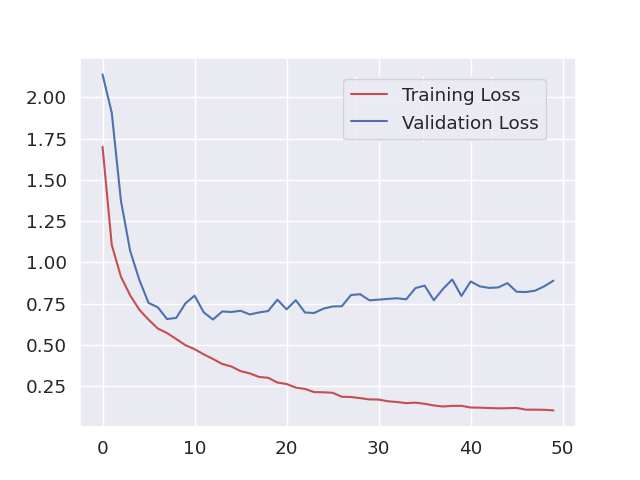
\includegraphics[scale=0.5]{fed_images/train_loss_MobileNetv2.png}
    \caption{The loss graph for the first successful training of MobileNetV2}
    \label{figure:loss_mnv2}
\end{figure}

The graph \ref{figure:loss_mnv2} illustrates the training and validation loss for the MobileNetV2 model. As training progresses, both losses decrease sharply, demonstrating that the model is learning from the data. Around the 20-epoch mark, the training loss continues to decline steadily, indicating that the model is fitting well to the training data. The validation loss begins to see a slight upward trend after around 11 epochs suggesting that the model is overfitting as the training loss continues to decrease.

\begin{figure}[H]
    \centering{}
    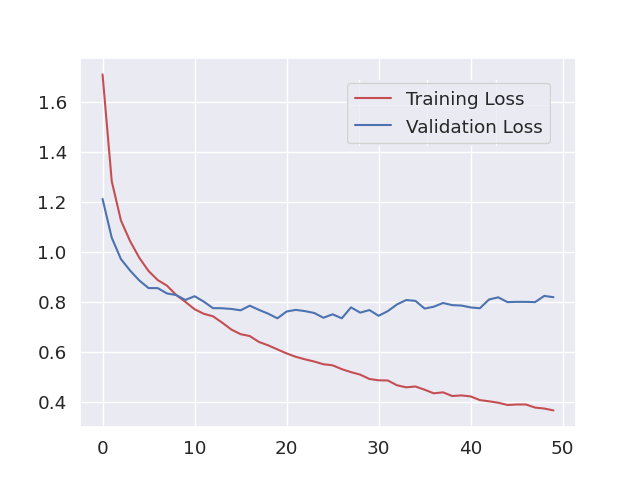
\includegraphics[scale=0.5]{fed_images/train_loss_ResNet50.png}
    \caption{The loss graph for the first successful training of ResNet50}
    \label{figure:loss_rn50}
\end{figure}

Graph \ref{figure:loss_rn50} shows the training and validation loss for the ResNet50 model. Similar to MobileNetV2, both losses start high and decrease significantly in the early epochs. The training loss for ResNet50 drops more quickly and smoothly compared to the validation loss, reaching a much lower value as epochs progress. The validation loss shows a decreasing trend but with more pronounced fluctuations, indicating some instability in performance on the validation set. After around 30 epochs the validation loss starts a slight upward trend. By the end of the 50 epochs, the training loss is significantly lower than the validation loss, which might suggest slight overfitting.

\begin{figure}[H]
    \centering{}
    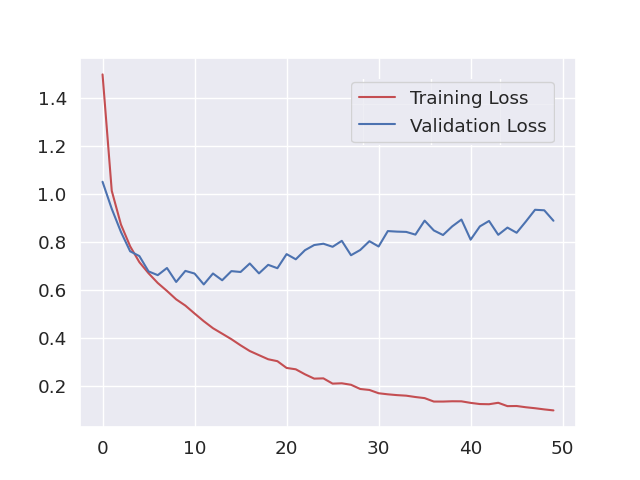
\includegraphics[scale=0.5]{fed_images/train_loss_VGG16.png}
    \caption{The loss graph for the first successful training of VGG16}
    \label{figure:loss_vgg16}
\end{figure}

Finally, graph \ref{figure:loss_vgg16} represents the training and validation loss for the VGG16 model. Both losses start high and decrease rapidly in the initial epochs, similarly to the other models. However, the training loss for VGG16 continues to decrease more steeply and steadily, reaching very low values, indicating a strong fitting to the training data. The validation loss decreases initially but starts to exhibit more fluctuation and even an upward trend after around 11 epochs. This divergence between training and validation loss suggests that VGG16 might be overfitting to the training data, capturing noise and details that do not generalise well to the validation set.

To further mitigate the impact of overfitting in the three emotion recognition models a few more techniques were added. Firstly an early stopper was added, this, with a patience set at 10, stops the training of the model if no improvements are made after 10 epochs of training and a checkpointer that will restore the model to the best weights. Alongside this, a reduced learning rate was implemented that lowers the learning rate if the training starts to hit a plateau in accuracy.

\begin{figure}[H]
    \centering{}
    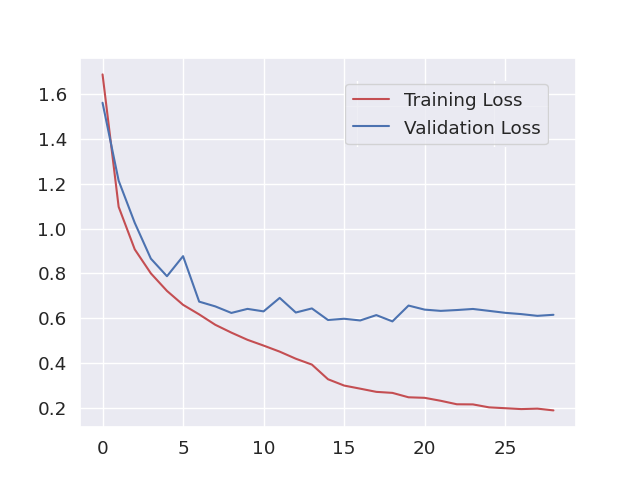
\includegraphics[scale=0.5]{fed_images/train_loss_MobileNetv2_ofp.png}
    \caption{The loss graph for the second successful training of MobileNetV2}
    \label{figure:loss_mnv2_ofp}
\end{figure}

MobileNetV2s second training loss graph is shown in figure \ref{figure:loss_mnv2_ofp}. The graph shows that the training only got to 29 epochs before the early stopper function stopped it. The application of techniques to prevent overfitting seems effective. The gap between training and validation loss is relatively small. The model continues to improve on both training and validation data, indicating that it is learning useful patterns rather than just memorising the training data. The stabilisation of the validation loss suggests that the model has reached a point where further training may yield diminishing returns.

\begin{figure}[H]
    \centering{}
    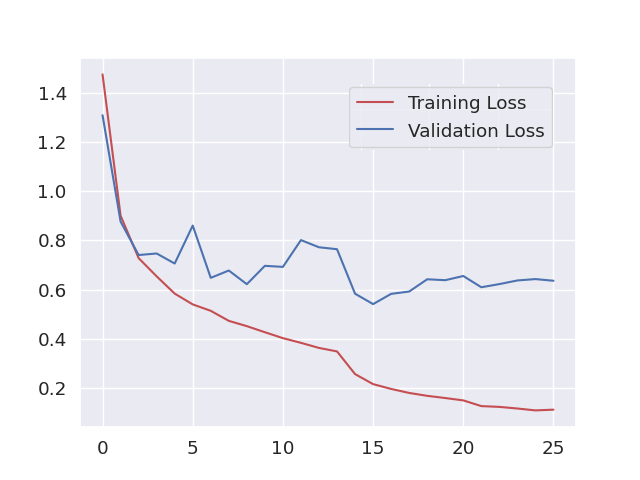
\includegraphics[scale=0.5]{fed_images/train_loss_ResNet50_ofp.png}
    \caption{The loss graph for the second successful training of ResNet50}
    \label{figure:loss_rn50_ofp}
\end{figure}

ResNet50's second training results in a similar graph to its first run. After only 5 epochs validation loss begins to fluctuate increasing and decreasing until around epochs 15 to 25, where the validation loss shows a slight upward trend.

\begin{figure}[H]
    \centering{}
    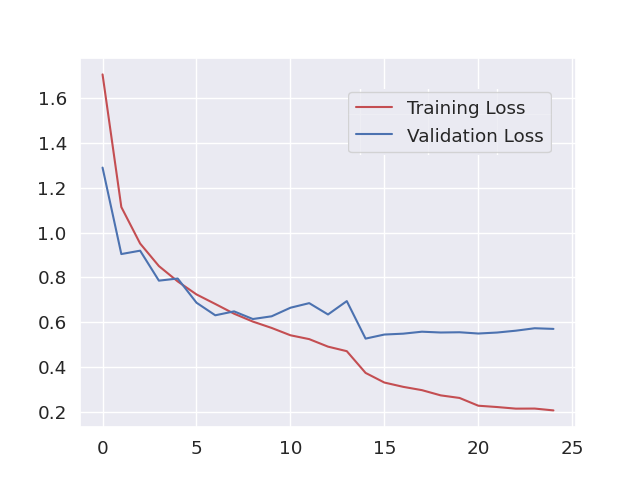
\includegraphics[scale=0.5]{fed_images/train_loss_VGG16_ofp.png}
    \caption{The loss graph for the second successful training of VGG16}
    \label{figure:loss_vgg16_ofp}
\end{figure}

In the second training run of VGG16 after about 5 epochs, the validation loss begins to fluctuate, while the training loss continues to decrease steadily. From Epochs 10 to 25, the validation loss shows a slight downward trend with occasional fluctuations, indicating potential minor overfitting. However, the training loss continues to decrease smoothly, suggesting that the model is still learning effectively. Overall, the model demonstrates good generalisation, and the techniques applied seem to mitigate the severe overfitting it saw in the first run.

\begin{figure}[H]
    \centering{}
    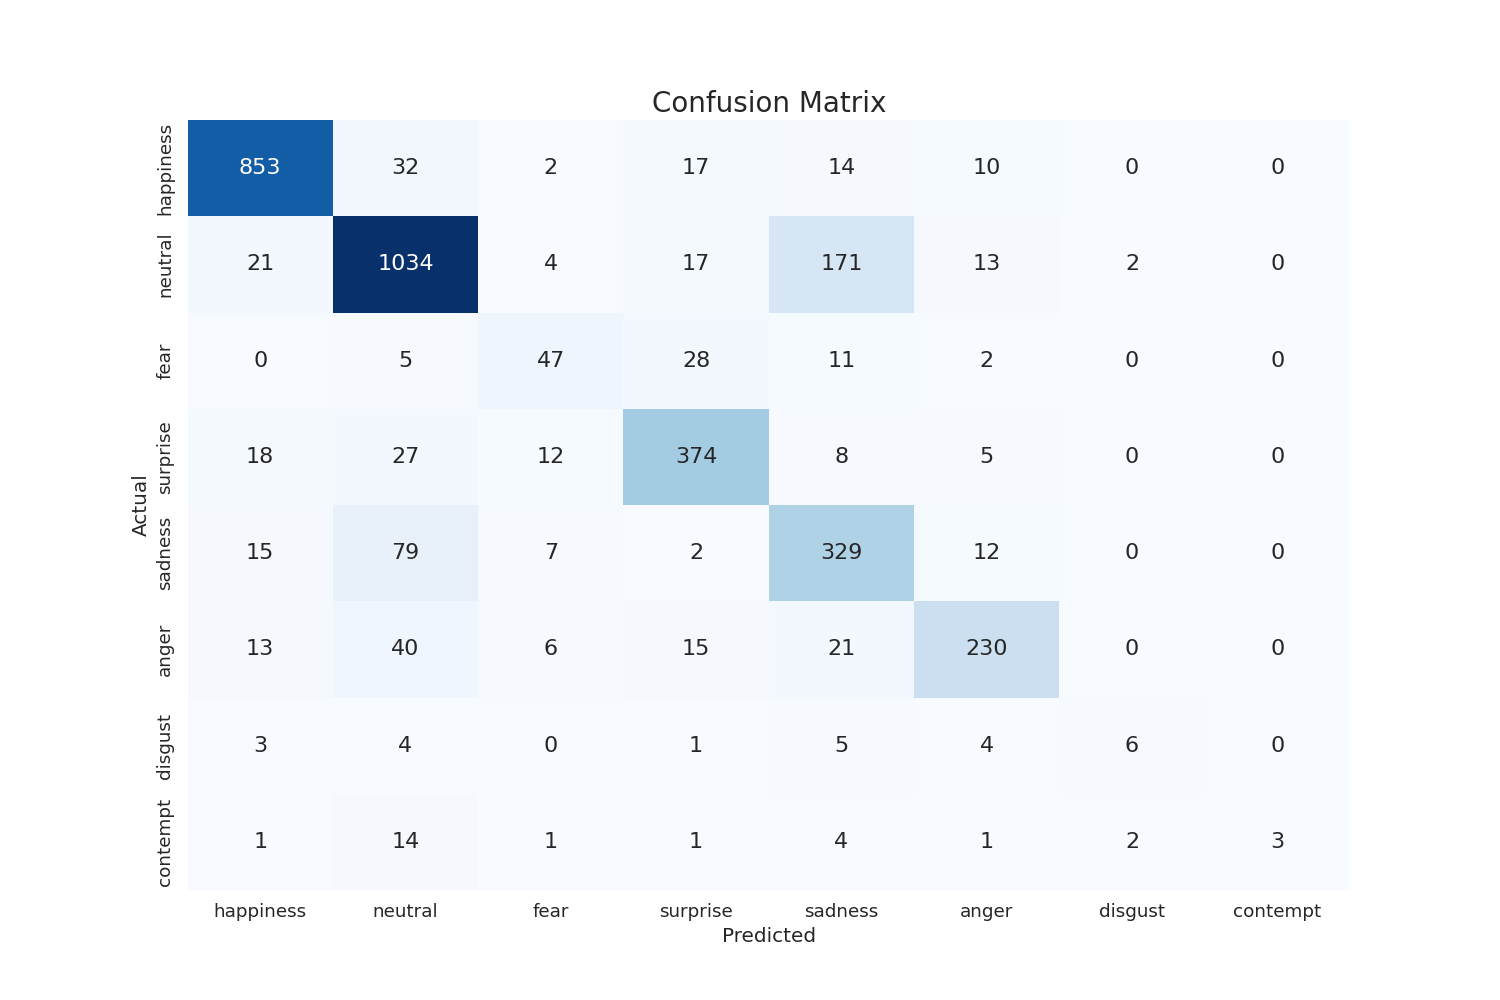
\includegraphics[scale=0.38]{fed_images/conf_matrix_MobileNetv2.png}
    \caption{The confusion matrix detailing the performance of MobileNetV2 on the PrivateTest set}
    \label{figure:conf_mnv2}
\end{figure}

The confusion matrix \ref{figure:conf_mnv2} illustrates the performance of MobileNetV2 across the 8 emotions. The model accurately classifies the `happiness' and `neutral' expressions, with 853 and 1034 correct predictions, respectively. However, it struggles with `fear' and `contempt' frequently misclassifying them as other emotions. There is notable confusion between `sadness' and `neutral' with it incorrectly classifying them as each other.

Figure \ref{figure:sadneutral} shows an example of images from sadness and neutral. The confusion could be attributed to the subtle facial differences between `sadness' and `neutral' expressions. Both emotions tend to exhibit minimal facial muscle movement, and the lack of exaggerated features such as smiles or frowns can make it challenging for models to distinguish between them.

\begin{figure}[H]
    \centering{}
    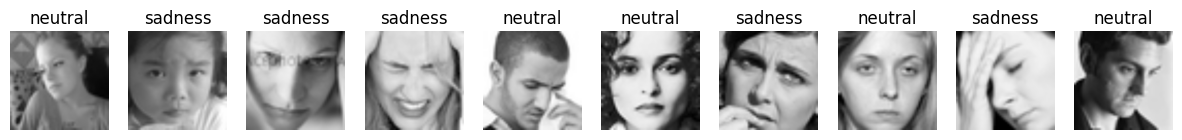
\includegraphics[scale=0.38]{fed_images/sadness+neutral.png}
    \caption{Example images showing the very slight variation between sadness and neutral}
    \label{figure:sadneutral}
\end{figure}

\begin{figure}[H]
    \centering{}
    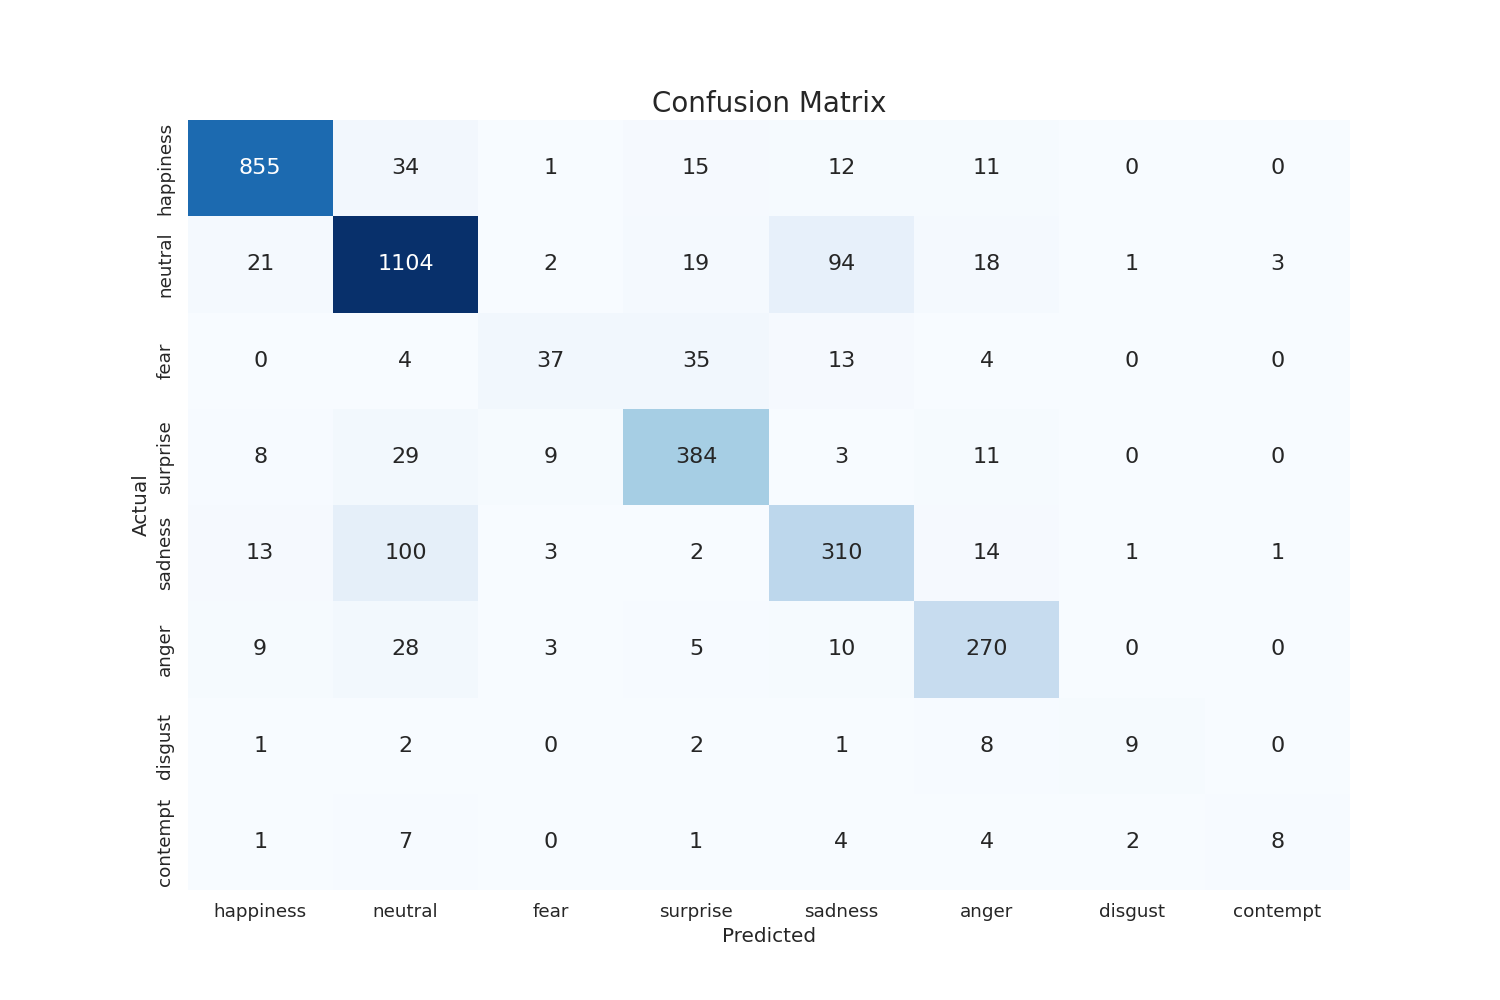
\includegraphics[scale=0.38]{fed_images/conf_matrix_ResNet50.png}
    \caption{The confusion matrix detailing the performance of ResNet50 on the PrivateTest set}
    \label{figure:conf_rn50}
\end{figure}

ResNet50 performed very similarly to MobileNetV2 but had a slightly higher recognition rate for each emotion except `fear' and `sadness'. It suffers from the same misclassification of `sadness' and `neutral' as MobileNetV2.

\begin{figure}[H]
    \centering{}
    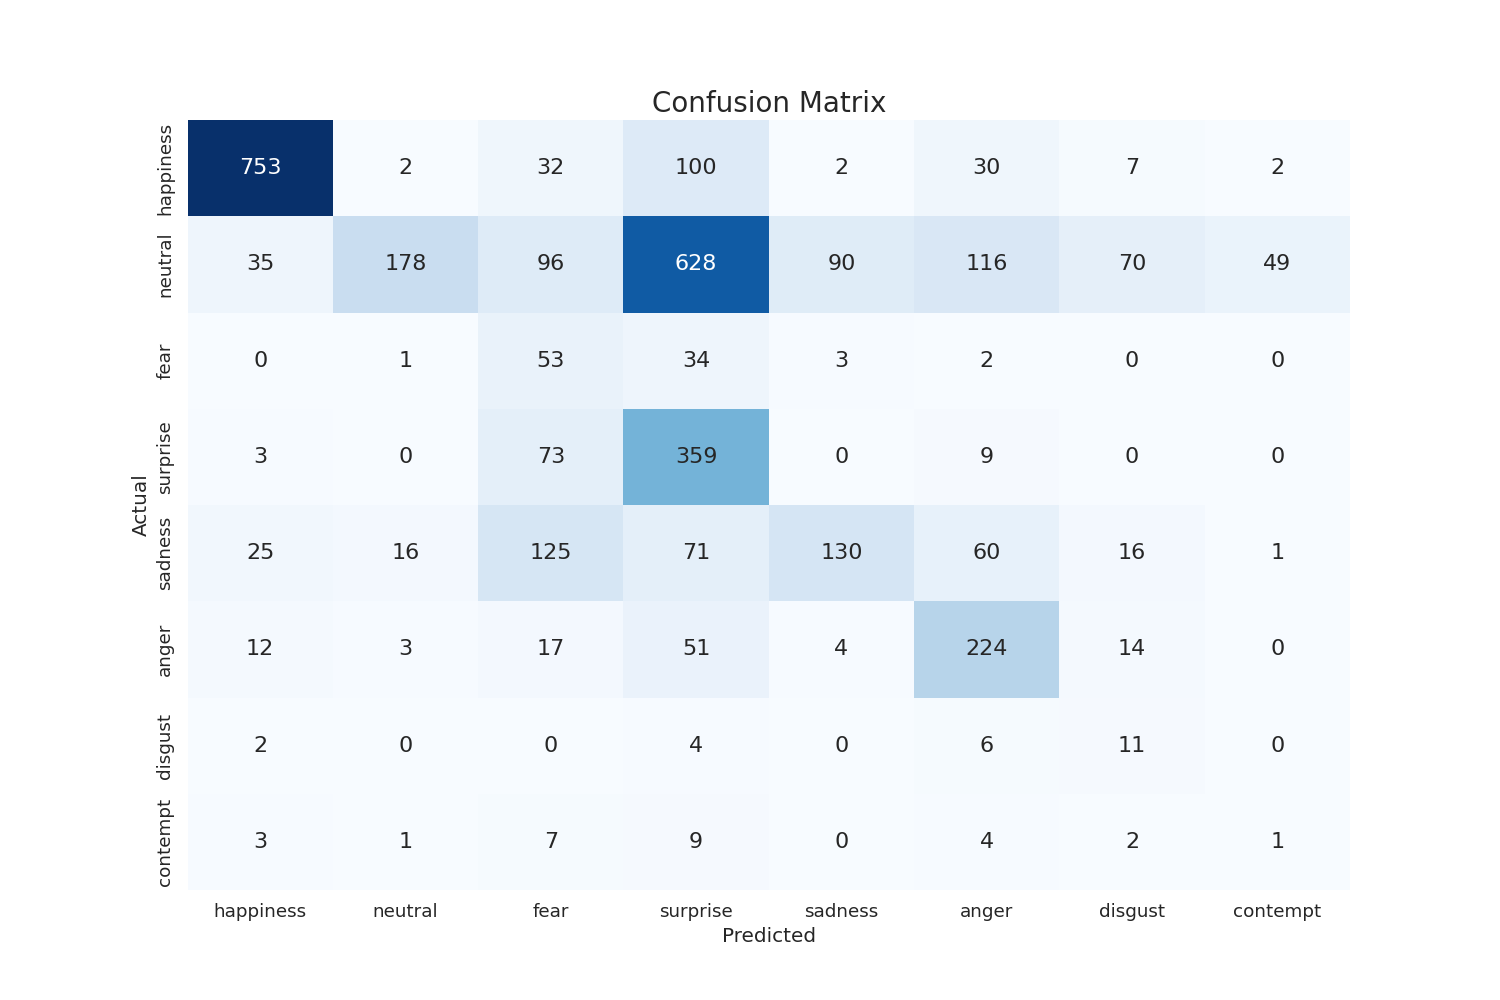
\includegraphics[scale=0.38]{fed_images/conf_matrix_VGG16.png}
    \caption{The confusion matrix detailing the performance of VGG16 on the PrivateTest set}
    \label{figure:conf_vgg16}
\end{figure}

VGG16 misclassified most of the `neutral' pictures, only getting 178 correct, mainly classifying them as `surprise' and `anger'. However, VGG16 achieved the highest results of the three models in the fear category. The model also struggles to differentiate between `sadness' and `fear'. Overall, the model does perform well; however, in comparison to ResNet50 and MobileNetV2, it misclassifies too many emotions to be considered reliable.

\subsection{Testing Combined Face and Emotion Recognition}

This section evaluates the performance of three emotion recognition models in conjunction with face detection algorithms: Haar cascades, dlib, Tiny YOLO and YOLO. The evaluation is conducted using the Expression in-the-Wild (ExpW) dataset, which contains facial images captured in diverse and unconstrained environments. This comprehensive testing aims to assess the robustness and accuracy of the models and algorithms in recognising emotions under varied and challenging scenarios.

To determine the optimal combination of face detection and emotion detection algorithms for use in a resource-constrained robotic system, a comprehensive test was performed. This test involved pairing each face detection algorithm with each emotion detection algorithm to evaluate their performance. The primary goal was to find the best performing combination in terms of speed and accuracy for real-time applications on the robot. Each face detection and emotion detection instance was measured to calculate the average time taken for detection and prediction. Successful detections of faces and correct emotion predictions were meticulously recorded and compared to the actual emotions presented in the images of the data set.

\begin{table}[h!]
\centering{}
\caption{Average Detection Times in Milliseconds for Face and Emotion Detection Algorithms}
\begin{tabular}{|l|l|c|c|}
\hline
\textbf{Algorithm} & \textbf{Algorithm Name} & \textbf{Avg. Inf Time (ms)} & \textbf{Model Size (MB)}\\ \hline
\textbf{Face} & Tiny YOLO               & 25.0    &   22.4                                            \\ \cline{2-4}
                        & Haar Cascade            & 40.7    &   1.19                    \\ \cline{2-4}
                        & dlib                    & 45.6    &   0.696                   \\ \cline{2-4}
                        & YOLO                    & 161.0   &   244                     \\ \hline
\textbf{Emotion} & MobileNetV2          & 13.6    &   69.8                                            \\ \cline{2-4}
                        & ResNet50                & 95.3    &   187                      \\ \cline{2-4}
                        & VGG16                   & 312.2   &   80.8                     \\ \hline
\end{tabular}
\label{tab:algorithm_detection_times_ms}
\end{table}


\begin{table}[h!]
\centering{}
\caption{Accuracy and Number of Face Detection for Model Combinations, out of a possible 91,793 faces}
\begin{tabular}{|l|c|c|}
\hline
\textbf{Model Combination}   & \textbf{Accuracy} & \textbf{No.\ of Face Detections} \\ \hline
dlib + MobileNetV2           & 37.06\%           & 56098                                   \\ \hline
dlib + ResNet50              & 37.77\%            & 56098                                   \\ \hline
dlib + VGG16                 & 34.52\%            & 56098                                   \\ \hline
Haar + MobileNetV2           & 46.63\%            & 76416                                   \\ \hline
Haar + ResNet50              & 47.81\%            & 76416                                   \\ \hline
Haar + VGG16                 & 44.52\%            & 76416                                   \\ \hline
Tiny YOLO + MobileNetV2      & 55.93\%            & 88332                                   \\ \hline
Tiny YOLO + ResNet50         & 57.36\%            & 88332                                   \\ \hline
Tiny YOLO + VGG16            & 51.94\%            & 88332                                   \\ \hline
YOLO + MobileNetV2           & 57.54\%            & 90773                                   \\ \hline
YOLO + ResNet50              & 59.02\%            & 90773                                   \\ \hline
YOLO + VGG16                 & 53.43\%            & 90773                                   \\ \hline
\end{tabular}
\label{tab:model_combinations_accuracy}
\end{table}

Since only one face in each image is annotated, all faces detectable in the image are compared to the one in the labels file, and the detected face that is closest (using Euclidian distance) to the listed face is considered the valid face for further analysis.

Tiny YOLO and YOLO, as face detection methods, provide the highest number of face detections, leading to improved overall accuracy when combined with emotion recognition models. Specifically, YOLO paired with ResNet50 achieves the highest accuracy in emotion recognition (59.02\%). Haar Cascade and dlib both achieved a lower number of face detections (resulting in lower overall accuracy) and a slower detection speed than Tiny YOLO which achieved a detection time of 0.0250 seconds on average. YOLO does provide a higher accuracy when it comes to the number of face detections and as a result, a higher overall accuracy; however, this increase in accuracy comes at the downside of 0.1610 seconds per face detection, more than 6 times slower than its Tiny counterpart for an overall accuracy increase of only 1.66\%. Thus, Tiny YOLO is the clear choice for facial recognition models. Among the emotion recognition models, ResNet50 generally outperforms MobileNetV2 and VGG16 across all face detection methods; however, considering the difference in detection times for ResNet50 (95.3 milliseconds) and MobileNetV2 (13.6 milliseconds) the choice is not as obvious and both could be left as suitable options depending on the need for higher accuracy or higher detection speed. Another consideration in a resource-constrained environment is the size of the models. ResNet50 has the largest model size at 187MB leaving less memory for the robots other processes to work with. This leaves the best combination for overall accuracy, memory efficiency, and speed to be Tiny YOLO + MobileNetV2 with it only requiring 92.2 MB of memory for both models.

Finally, the performance of the model is evaluated directly on a robot. The system is designed to be standalone and operate without relying on a connected PC, so testing the models in this context is essential.

\begin{table}[h!]
\centering{}
\caption{Average Detection Times in Milliseconds for Face and Emotion Detection Algorithms performed on the TurtleBot4}
\begin{tabular}{|l|l|c|}
\hline
\textbf{Algorithm Type} & \textbf{Algorithm Name} & \textbf{Average Detection Time (ms)} \\ \hline
\textbf{Face Detection} & Tiny YOLO               & 697.4                                \\ \cline{2-3}
                        & Haar Cascade            & 491.7                                \\ \cline{2-3}
                        & dlib                    & 216.2                                \\ \cline{2-3}
                        & YOLO                    & 6846.5                               \\ \hline
\textbf{Emotion Detection} & MobileNetV2          & 124.7                                \\ \cline{2-3}
                        & ResNet50                & 1334.3                               \\ \cline{2-3}
                        & VGG16                   & 5384.2                               \\ \hline
\end{tabular}
\label{tab:algorithm_detection_times_ms_robot}
\end{table}

The results of the Turtlebot4 tests are summarised in the table above. It should be noted that the performance of face detection methods exhibits a significant reversal when implemented on a robot with limited resources. Surprisingly, Tiny YOLO, which was initially the fastest, was surpassed by both dlib and Haar Cascade. Even Haar Cascade, was outperformed by dlib by a considerable margin. This behaviour could be due to a couple things, the Turtlebot 4 does not possess any GPUs unlike the training PC and it is possible that YOLO is using GPU acceleration to improve detection times. The other possibility is that YOLO leverages the vastly increased number of CPU cores on the training PC to perform parallel computations more efficiently, distributing the workload across multiple cores. However, when deployed on the Turtlebot4, which has significantly fewer cores, YOLO's speed advantage diminishes, leading to slower inference times compared to simpler models like dlib and Haar Cascade.

The results for the emotion models remained consistent with the original tests conducted on the training PC. Among these models, MobileNetV2 stands out as the fastest and most accurate choice for direct implementation on a robot. However, the selection of a face detection model is more nuanced. For maximum accuracy, Tiny YOLO is the preferred option, closely trailing full YOLO in accuracy, but with each detection taking less than a second as opposed to 6.8 seconds. If rapid detections are a priority, dlib is a clear choice, while Haar Cascade provides a balanced compromise between accuracy and inference speed.

\section{Sentiment Analysis}

This chapter examines the audio emotion recognition component of the multimodal framework, focusing on the use of IBM Watson's capabilities. The analysis includes performance tests to assess the accuracy and speed of IBM Watson in detecting emotions from audio input. Additionally, this chapter discusses the role of large language models (LLMs) in the context of emotion recognition and the limitations that prevent the use of OpenSMILE for this project. Through a detailed evaluation, this chapter aims to provide insight into the effectiveness of IBM Watson as an audio emotion recognition tool and the considerations involved in choosing appropriate technologies for audio analysis.

\section{IBM Watson}

Given the current computational demands of core functionalities and concurrent facial emotion recognition processes, it would be beneficial to consider offloading speech emotion recognition to an external entity. Using cloud-based solutions, such as IBM Watson's API, presents an appealing option. By interfacing with Watson, recorded human speech can be remotely processed, allowing emotional predictions based on textual analysis. This approach not only reduces the computational burden on the robot, but also harnesses the advanced emotion analysis capabilities offered by cloud services.

IBM Watson is a cognitive computing platform developed by IBM that uses artificial intelligence (AI) techniques to analyse and interpret large amounts of data. It includes a range of AI-powered services and tools designed to help businesses gain insights, make informed decisions, and improve user experiences in various industries. Watson's capabilities include natural language processing, machine learning, and data analytics, making it a versatile solution for addressing complex challenges.

One useful feature of IBM Watson is its conversational abilities, which allow for structured dialogue between the robot and the user. By integrating Watson's Conversation service, the robot can engage in structured conversations with users, responding to prompts and queries based on predefined conversation trees. This approach allows the robot to guide the conversation along predetermined paths, collecting specific information, or addressing user inquiries within predefined topics.

Ultimately, the choice to use cloud-based emotion recognition is a strategic decision that weighs computational efficiency against the aim of developing a flexible and emotionally intelligent robotic system. By tapping into external resources, we not only enhance the robot's performance but also pave the way for integrating state-of-the-art emotion analysis capabilities into the HRI framework, thereby enhancing the user experience and pushing the boundaries of human-robot interaction. \cite{Kumar2022-gd}

Initially, a system was created to incorporate IBM Watson as a chatbot to inform people about ongoing public health issues. The goal was to provide accurate and up-to-date responses to common questions and to give people peace of mind. The system was designed to use IBM’s sentiment analysis to detect fear and point people to resources that could help them. In addition, the chatbot provided the ability to connect an Aldebaran robot, which provided a physical presence that people could interact with. The robot would use its microphones to pick up user speech, which could then be sent to IBM for analysis, after which the robot would respond with what IBM Watson sent back.

\begin{figure}[!htb]
    \centering{}
    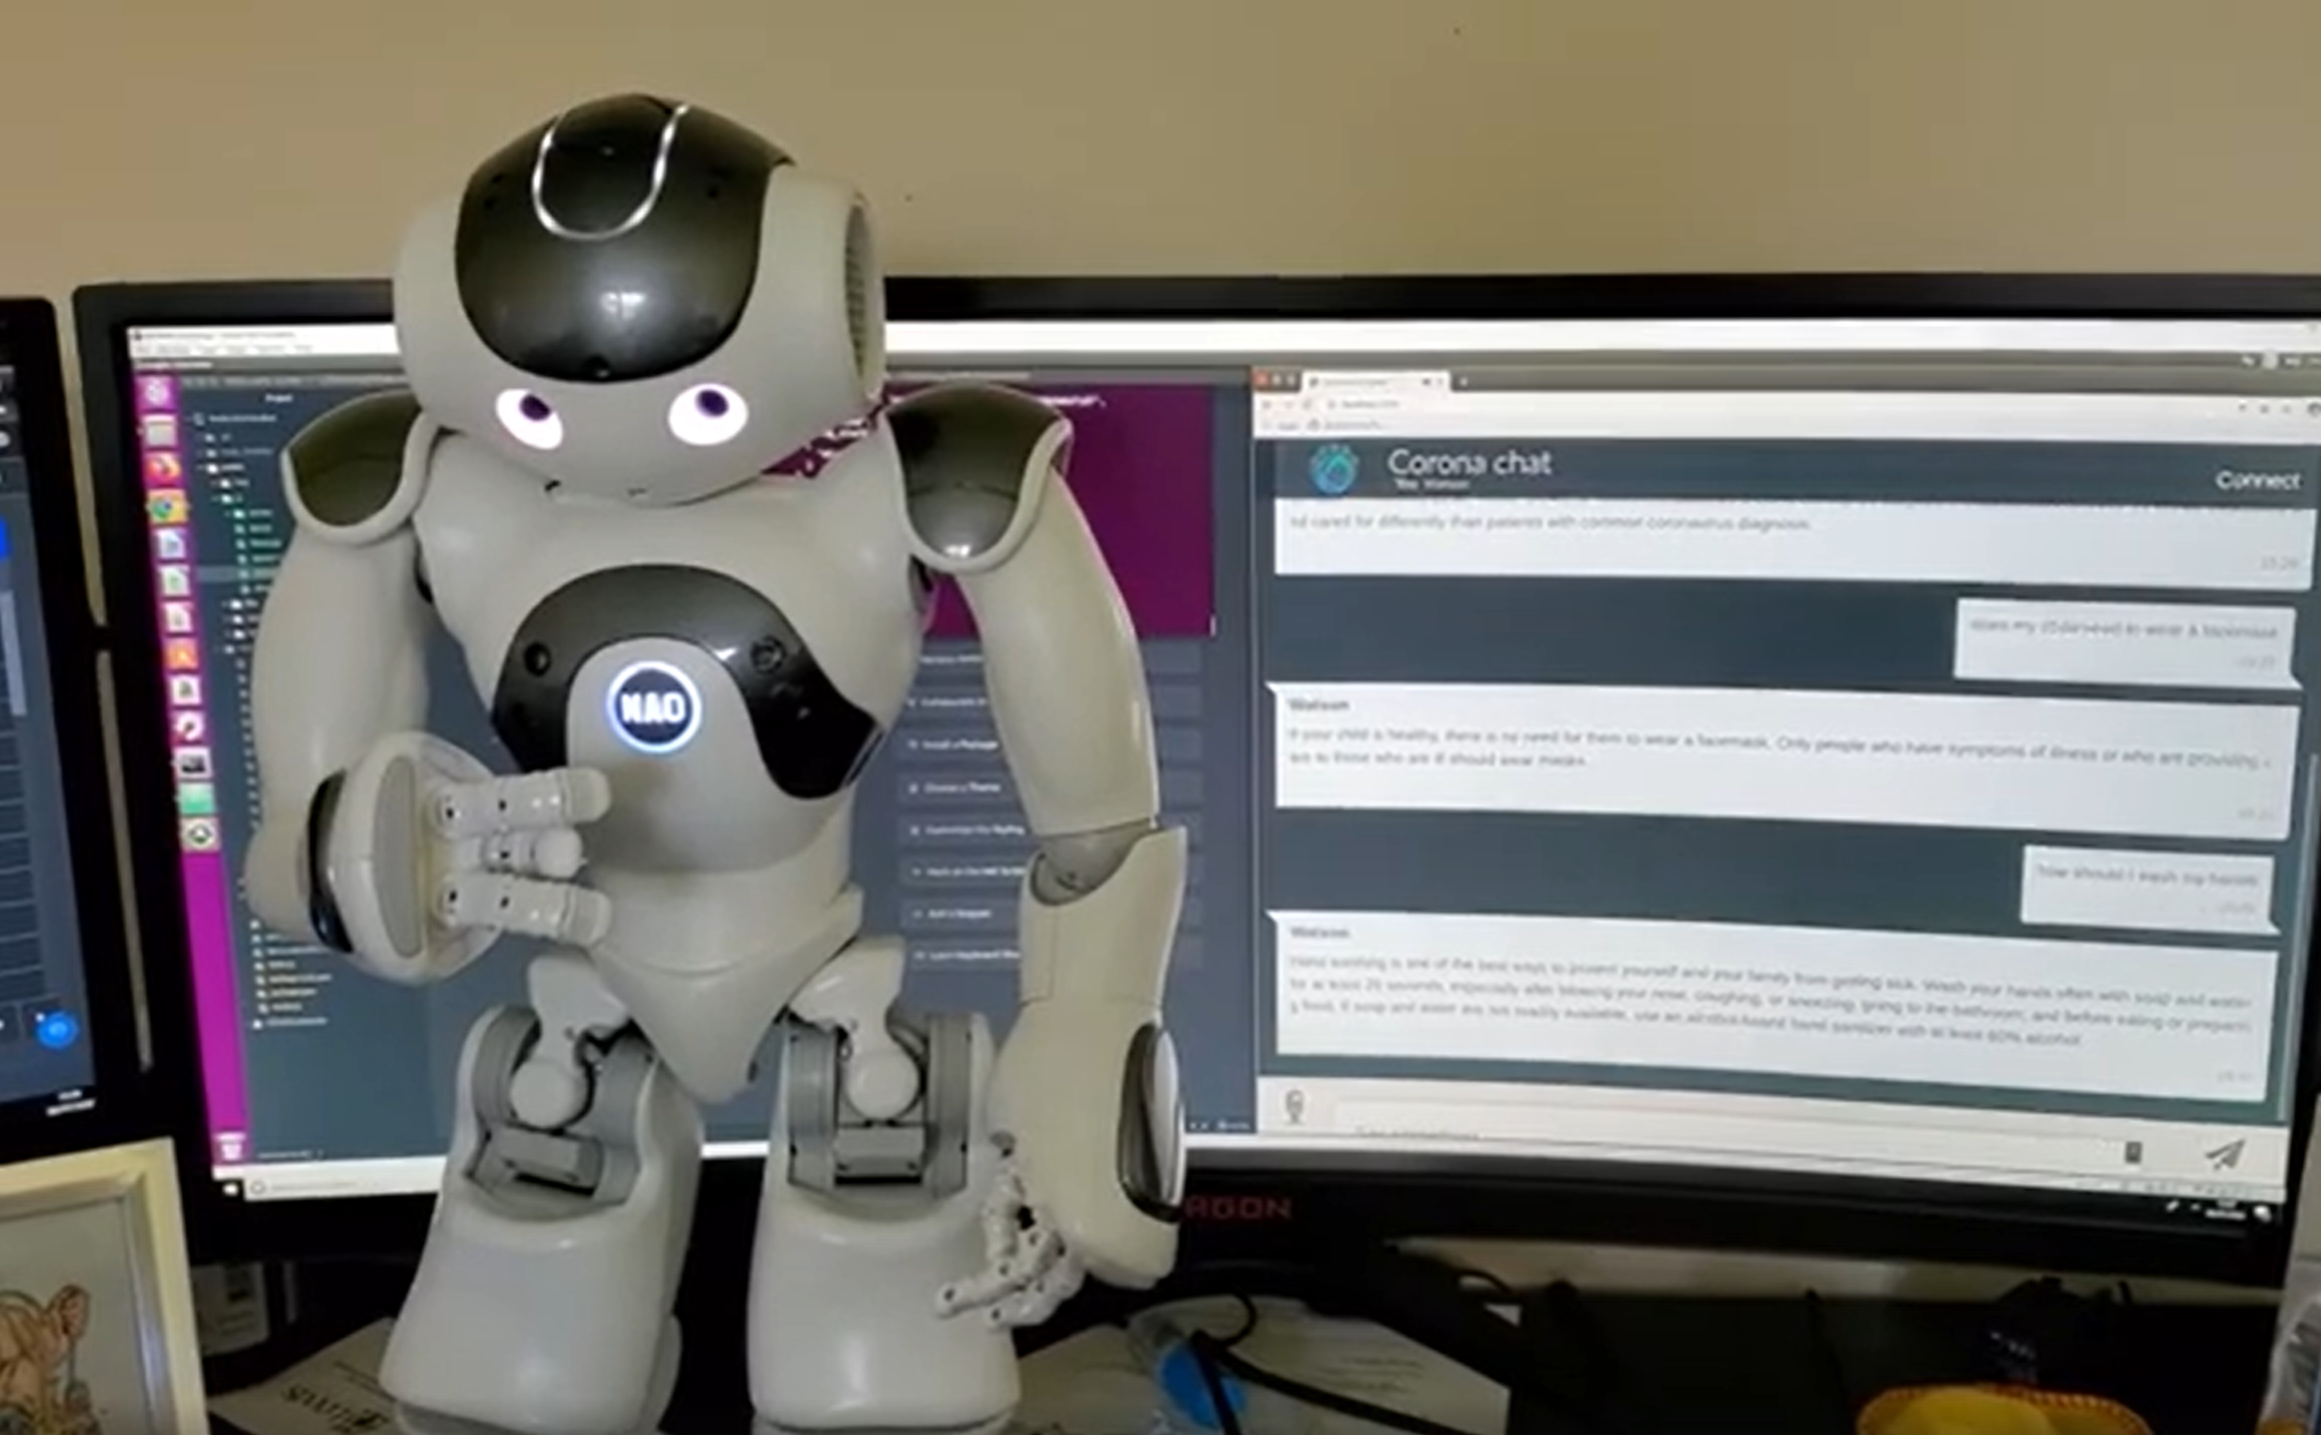
\includegraphics[scale=0.25]{aed_images/nao_with_chatbot.png}
    \caption{Aldebaran robot Nao with IBM Watson ChatBot}
    \label{figure:naochatbot}
\end{figure}

This system also leveraged IBM Watson's text-to-speech capabilities, allowing users to fully customise the generated voice based on a variety of parameters. In addition to selecting the gender of the voice, users could choose accents from different regions, making the interaction more personalised and culturally relevant. This also allows adjustments to pitch, enabling a higher or lower tone depending on user preference or specific application needs.

\section{LLM}

It is important to note that while IBM Watson's Conversation service provides a structured approach to dialogue management, it may lack the spontaneity and flexibility of natural human conversation. Relying on conversation trees imposes constraints on the flow of interaction, limiting the opportunity for open-ended dialogue and real-time adaptation to user input. As a result, interactions with the robot may feel scripted or constrained, potentially detracting from the overall user experience in certain situations.

To achieve a natural and engaging human-robot interaction, it is imperative to develop a comprehensive system that integrates a Large Language Model (LLM). ChatGPT, a state-of-the-art language model, plays a crucial role in enabling seamless human-like conversations between the robot and the user \cite{chatgpt}. Its ability to generate contextually relevant responses allows for a more natural dialogue exchange that closely resembles human conversation patterns.

By incorporating ChatGPT into this system, we can create a more interactive and emotionally responsive dialogue experience. In this setup, the speech-emotion recognition system handles the analysis of user speech to detect emotions such as happiness, sadness, anger, or neutrality. These detected emotional states can then be communicated to ChatGPT alongside the text of the user's speech. This allows ChatGPT to factor in both the content of the conversation and the emotional context provided by the speech-emotion recognition system, helping it generate more empathetic and contextually appropriate responses.

For example, if the speech-emotion recognition system detects frustration in the user's voice, this emotional information can be fed to ChatGPT, allowing it to adapt its responses in real time to address the user’s emotional state more sensitively. This synergy allows for a deeper and more emotionally aware interaction, where ChatGPT can tailor the flow of the conversation based on both the user’s words and their emotional tone.

Additionally, ChatGPT can use the emotional feedback from the speech-emotion system to adjust the direction of the conversation, perhaps steering toward topics that might alleviate negative emotions or enhance positive ones. This makes it possible to create a more engaging and emotionally intelligent interaction, where the robot can respond in a way that feels more human and responsive to the user's mood. Using ChatGPT for dialogue and the emotion recognition system for emotional analysis, we enable a hybrid approach where each component focuses on its strengths, resulting in a more robust and user-centric interaction.

Thus, ChatGPT was integrated into the system. This allows users to interact with ChatGPT seamlessly through a browser, making it accessible from virtually any device, whether a desktop, laptop, or mobile device. This integration ensures that users can engage with the system without the need for specialised software or hardware, broadening its utility and accessibility. The Web Messenger supports both text- and speech-based interactions allowing the user to converse with the robot in a natural way.

One of the core strengths of this system lies in how it expands ChatGPT's capabilities, making it a far more versatile assistant. Using the function-calling mechanism, ChatGPT can now fetch real-time data such as weather reports, time, and date, or even retrieve specific data from databases. This transforms it from being a static question-answering system to an interactive, real-time assistant. Moreover, the system has been designed to allow future scalability, enabling developers to integrate additional functions based on evolving user needs, such as connecting to more advanced AI models, adding new APIs, or enhancing its conversational context-awareness.

The system could also leverage locally run language models, such as GPT4All, to enhance its natural language understanding and response capabilities. Running these models locally ensures full control over data privacy and security. This approach allows for greater flexibility, as the models can be fine-tuned to better suit the system's specific needs without reliance on external cloud services. In addition, the system can operate independently of an internet connection, making it more reliable in environments with limited or unstable connectivity. This setup offers both customisation options and scalability, ensuring robust performance for complex, language-driven tasks.

\section{OpenSMILE}

OpenSMILE \cite{opensmile-2010}, which stands for ``Open-Source Speech and Music Interpretation by Large-Space Extraction'' is a powerful open-source toolkit widely used in audio signal processing. Its primary function is to extract an extensive range of acoustic features from audio signals, providing a versatile platform for various applications that include speech recognition, emotion recognition, speaker identification, and music analysis. One of the key strengths of OpenSMILE lies in its modular architecture, which allows the customisation of the feature extraction process to suit specific requirements. This modularity is achieved through a collection of feature extraction components known as ``functionals'' each responsible for computing a particular set of features. It is possible to choose from a rich library of functionals and combine them as needed to create tailored feature sets.

Moreover, OpenSMILE is designed for real-time processing of audio streams, making it suitable for applications that demand low-latency feature extraction, such as real-time speech recognition systems or interactive multimedia applications. Its cross-platform compatibility ensures that it can seamlessly integrate into various environments running on major operating systems, including Windows, macOS, and Linux. Additionally, the toolkit offers extensive configuration options that allow one to specify parameters such as frame size, overlap, and feature selection, thus providing flexibility to adapt to various audio processing tasks.

OpenSMILE facilitates the integration of extracted features with machine learning algorithms, serving as a crucial preprocessing step for tasks such as classification. The features computed by OpenSMILE capture essential characteristics of audio signals, enabling accurate modelling and interpretation of audio data. However, given the limited resources available on a robotic platform, it could run into performance issues that severely limit its capabilities. The memory requirements of OpenSMILE can also be significant, particularly when extracting a large number of features from lengthy audio streams, with each feature set taking up to 100MB for a short 18-second audio clip. Robotics platforms typically have limited memory capacity, and allocating resources to OpenSMILE may strain the system, potentially impacting overall system stability and reliability. This limitation is purely hardware based and future robots that can afford more powerful systems would be able to utilise OpenSMILE feature extraction plus a classification model to determine emotions.

\section{IBM Waston Performance}

In this section, the performance of IBM Watson's Natural Language Understanding (NLU) service is evaluated in analysing the emotional content of various phrases. To ensure a robust assessment, each phrase was tested five times, and response times were recorded. The table \ref{tab:phrase_tests} presents the response times (in seconds) for each test run with ten different phrases shown in \ref{tab:phrases_emotions}.

\begin{table}[h!]
\centering{}
\caption{Phrases and their expected emotions}
\begin{tabular}{|p{9cm}|c|}
\hline
\textbf{Text} & \textbf{Expected Emotion} \\ \hline
I am so happy today! Everything is going great. & Joy \\ \hline
I am very sad and disappointed by the news. & Sadness \\ \hline
I am so angry at the situation! & Anger \\ \hline
This is so scary and frightening. & Fear \\ \hline
I am just so disgusted by what happened. & Disgust \\ \hline
The sun is shining and the birds are singing. It's a beautiful day to be alive. I feel so grateful for all the wonderful things in my life. I have a loving family, great friends, and a job that I am passionate about. Days like today make me feel like all the hard work has paid off and I can truly appreciate the beauty of life. & Joy \\ \hline
Today I received some heartbreaking news. A dear friend of mine passed away unexpectedly. The shock and sorrow I feel are overwhelming. We had so many plans together, so many dreams left unfulfilled. It's hard to imagine life without them. This loss leaves a void that can never be filled. & Sadness \\ \hline
I am furious about the latest policy changes at work. They were implemented without any consultation with the staff, and they make our jobs much harder. It feels like management doesn't care about our well-being or input. This kind of disregard is unacceptable, and I won't stand for it. & Anger \\ \hline
Walking through the dark alley, I could feel my heart racing. Every sound seemed amplified, and the shadows looked like they were moving. I couldn't shake the feeling that someone was following me. It was one of the most terrifying experiences I've ever had. I just wanted to get out of there as quickly as possible. & Fear \\ \hline
The food at that restaurant was absolutely disgusting. The meat was undercooked, the vegetables were soggy, and there was a strange smell coming from the kitchen. I felt nauseous just being there. It's unacceptable to serve such poor quality food to customers. & Disgust \\ \hline
\end{tabular}
\label{tab:phrases_emotions}
\end{table}
\clearpage{}

\begin{table}[h!]
\centering{}
\caption{Test results for IBM Watson's response times on 10 phrases across 5 runs in seconds, alongside the average time and standard deviation. The phrases in this table match the phrases in table \ref{tab:phrases_emotions} in order.}
\begin{tabular}{|c|c|c|c|c|c|c|c|}
\hline
\textbf{Test number} & \textbf{Run 1} & \textbf{Run 2} & \textbf{Run 3} & \textbf{Run 4} & \textbf{Run 5} & \textbf{Average} & \textbf{SD} \\ \hline
\textbf{Phrase 1}    & 1.81 & 2.07 & 1.36 & 1.58 & 1.45 & 1.654 & 0.257        \\ \hline
\textbf{Phrase 2}    & 0.69 & 0.51 & 0.38 & 0.40 & 0.36 & 0.468 & 0.123        \\ \hline
\textbf{Phrase 3}    & 0.43 & 0.47 & 0.39 & 0.36 & 0.40 & 0.41 &  0.037       \\ \hline
\textbf{Phrase 4}    & 0.69 & 0.63 & 0.38 & 0.39 & 0.43 & 0.504 & 0.130        \\ \hline
\textbf{Phrase 5}    & 0.38 & 0.38 & 0.40 & 1.23 & 0.48 & 0.574 & 0.330        \\ \hline
\textbf{Phrase 6}    & 0.47 & 0.40 & 0.60 & 0.52 & 0.43 & 0.484 & 0.071        \\ \hline
\textbf{Phrase 7}    & 0.56 & 0.43 & 0.40 & 0.61 & 0.41 & 0.482 & 0.086        \\ \hline
\textbf{Phrase 8}    & 0.43 & 0.42 & 0.39 & 0.44 & 0.39 & 0.414 & 0.021        \\ \hline
\textbf{Phrase 9}    & 0.47 & 0.41 & 0.40 & 0.40 & 0.45 & 0.426 & 0.029        \\ \hline
\textbf{Phrase 10}   & 0.42 & 0.40 & 0.36 & 0.45 & 0.39 & 0.404 & 0.030        \\ \hline
\end{tabular}
\label{tab:phrase_tests}
\end{table}

IBM Watson NLU demonstrates efficient and consistent performance in emotion analysis, with response times typically under one second for any given phrase. However, there is a noticeable delay for the first phrase of each session, likely due to the system establishing an initial connection to IBM Watson. To investigate this, five additional tests were conducted with the phrases in reverse order. The first, more complex, phrase took an average of 1.3601 seconds to process, while subsequent phrases averaged just 0.3713 seconds. This indicates that the first phrase consistently experiences a longer response time. To optimise performance, it would be beneficial for the program to send a throwaway phrase to minimise delays for subsequent inputs.

\begin{table}[h!]
\centering{}
\caption{The resulting output probability for each emotion for each phrase. The phrases in this table match the phrases in table \ref{tab:phrases_emotions} in order.}
\begin{tabular}{|c|c|c|c|c|c|}
\hline
\textbf{Test number} & \textbf{Sadness} & \textbf{Joy} & \textbf{Fear} & \textbf{Disgust} & \textbf{Anger} \\ \hline
\textbf{Phrase 1} & 0.025 & 0.983 & 0.008 & 0.002 & 0.006 \\ \hline
\textbf{Phrase 2} & 0.960 & 0.014 & 0.025 & 0.017 & 0.008 \\ \hline
\textbf{Phrase 3} & 0.070 & 0.031 & 0.036 & 0.005 & 0.861 \\ \hline
\textbf{Phrase 4} & 0.017 & 0.003 & 0.999 & 0.006 & 0.010 \\ \hline
\textbf{Phrase 5} & 0.225 & 0.001 & 0.019 & 0.894 & 0.067 \\ \hline
\textbf{Phrase 6} & 0.093 & 0.921 & 0.009 & 0.004 & 0.011 \\ \hline
\textbf{Phrase 7} & 0.672 & 0.129 & 0.076 & 0.010 & 0.098 \\ \hline
\textbf{Phrase 8} & 0.309 & 0.150 & 0.089 & 0.038 & 0.212 \\ \hline
\textbf{Phrase 9} & 0.245 & 0.269 & 0.419 & 0.011 & 0.044 \\ \hline
\textbf{Phrase 10}& 0.390 & 0.026 & 0.131 & 0.452 & 0.067 \\ \hline
\end{tabular}
\label{tab:test_results}
\end{table}

Each row in table \ref{tab:test_results} shows the predicted probabilities for sadness, joy, fear, disgust, and anger for each phrase in table \ref{tab:phrases_emotions}. Overall, IBM Watson's predictions match well with the expected emotions. However, the only phrase that did not meet the expected emotion is the one about changes in workplace policies (phrase 8), which was predicted mainly as sadness when the expected emotion was anger, anger was the next highest prediction.

\section{ChatGPT Performance}

In this section, we evaluate the performance of several models, including GPT-3.5-turbo, GPT-4o, and GPT-4o-mini \cite{openai2024}, by measuring their response times to a set of predefined phrases. Each model was tested multiple times to ensure a thorough assessment of efficiency. The recorded response times (in seconds) for each test run are presented in three separate tables. This analysis aims to provide insights into the responsiveness of each model and compare their performance under consistent testing conditions.

This section also provides an overview of the key differences among three language models: GPT-3.5-turbo, GPT-4o, and GPT-4o Mini. Each model is built on advanced architectures, but they vary significantly in performance and intended use cases.

\subsection{GPT-3.5-turbo}

ChatGPT 3.5-turbo is based on the GPT-3.5 engine, which was trained on over 175 billion parameters. While it represents a significant advancement in natural language processing, it has notable downsides. One major issue is its accuracy and reliability; ChatGPT 3.5 is more prone to `hallucinations', which means it can generate incorrect or non-sensical information, especially when faced with ambiguous queries. These limitations can lead to inappropriate outputs, which may affect user trust and satisfaction. Despite these challenges, ChatGPT 3.5-turbo remains effective for many applications, such as basic content generation and straightforward chatbot interactions.

\begin{table}[h!]
\centering{}
\caption{Test results for GPT-3.5-turbo response times over 10 phrases, alongside the average time and standard deviation. The phrases in this table match the phrases in table \ref{tab:phrases_emotions} in order.}
\begin{tabular}{|c|c|c|c|c|c|c|c|}
\hline
\textbf{Test number} & \textbf{Run 1} & \textbf{Run 2} & \textbf{Run 3} & \textbf{Run 4} & \textbf{Run 5} & \textbf{Average} & \textbf{SD} \\ \hline
\textbf{Phrase 1} & 0.91 & 0.91 & 0.86 & 1.05 & 0.99 & 0.944 & 0.067          \\ \hline
\textbf{Phrase 2} & 0.65 & 0.69 & 0.82 & 0.91 & 0.85 & 0.784 & 0.098          \\ \hline
\textbf{Phrase 3} & 1.26 & 0.95 & 1.95 & 1.70 & 1.20 & 1.412 & 0.362          \\ \hline
\textbf{Phrase 4} & 1.24 & 1.41 & 1.54 & 1.31 & 1.09 & 1.318 & 0.152          \\ \hline
\textbf{Phrase 5} & 0.96 & 1.07 & 1.11 & 1.02 & 1.04 & 1.040 & 0.050          \\ \hline
\textbf{Phrase 6} & 3.33 & 2.96 & 3.57 & 1.67 & 3.06 & 2.918 & 0.659          \\ \hline
\textbf{Phrase 7} & 2.93 & 3.43 & 2.73 & 2.70 & 1.84 & 2.726 & 0.514          \\ \hline
\textbf{Phrase 8} & 1.69 & 1.94 & 1.30 & 1.55 & 2.06 & 1.708 & 0.272          \\ \hline
\textbf{Phrase 9} & 2.55 & 3.44 & 2.66 & 4.42 & 2.76 & 3.166 & 0.700          \\ \hline
\textbf{Phrase 10}& 1.10 & 1.46 & 1.80 & 1.62 & 1.45 & 1.486 & 0.231          \\ \hline
\end{tabular}
\label{tab:phrase_gpt3.5}
\end{table}

From the results, it is noticeable that shorter, simpler phrases (like Phrase 1 and Phrase 2) tend to have lower response times, averaging around 0.94 and 0.78 seconds, respectively. These phrases exhibit relatively low standard deviations, indicating stable performance between runs. As the complexity of the phrases increases, the response times also increase, as seen in phrases such as Phrase 6 and Phrase 9, which have significantly higher averages of 2.91 and 3.16 seconds, respectively. These more complex phrases also show greater variation between runs, reflected by higher standard deviations (e.g., 0.659 for Phrase 6 and 0.700 for Phrase 9), suggesting that complexity affects both the processing time and consistency.

Interestingly, certain phrases such as Phrase 3 and Phrase 7 also show a marked increase in response time and standard deviation, indicating that as the task becomes more complex, the model requires more time and produces more varied results. Overall, the data demonstrates that GPT-3.5-turbo's response times correlate with phrase complexity, with the model generally being faster on simpler phrases and taking longer on more intricate ones.

\subsection{GPT-4o}

GPT-4o is the full-fledged version of the GPT-4 architecture, representing a significant upgrade over GPT-3.5-turbo. This model features enhanced accuracy and reliability, being trained on more than a trillion parameters, which allows it to generate more precise responses and significantly reduce the likelihood of hallucinations. GPT-4o excels at understanding nuanced contexts and producing coherent, contextually appropriate text. In addition, it is designed for complex tasks that require high computational power, making it suitable for applications in industries such as finance, healthcare, and research, where precision and depth are crucial.

\begin{table}[h!]
\centering{}
\caption{Test results for GPT-4o response times over 10 phrases, alongside the average time and standard deviation. The phrases in this table match the phrases in table \ref{tab:phrases_emotions} in order.}
\begin{tabular}{|c|c|c|c|c|c|c|c|}
\hline
\textbf{Test number} & \textbf{Run 1} & \textbf{Run 2} & \textbf{Run 3} & \textbf{Run 4} & \textbf{Run 5} & \textbf{Average} & \textbf{SD} \\ \hline
\textbf{Phrase 1} & 1.63 & 1.00 & 0.86 & 0.83 & 1.31 & 1.126 & 0.304          \\ \hline
\textbf{Phrase 2} & 0.82 & 0.87 & 1.24 & 0.87 & 0.70 & 0.900 & 0.181          \\ \hline
\textbf{Phrase 3} & 0.86 & 1.36 & 1.37 & 1.24 & 2.00 & 1.366 & 0.367          \\ \hline
\textbf{Phrase 4} & 1.74 & 0.81 & 1.36 & 1.07 & 1.10 & 1.216 & 0.315          \\ \hline
\textbf{Phrase 5} & 0.80 & 5.37 & 1.05 & 0.82 & 0.96 & 1.800 & 1.787          \\ \hline
\textbf{Phrase 6} & 1.49 & 1.97 & 1.22 & 2.31 & 3.63 & 2.124 & 0.842          \\ \hline
\textbf{Phrase 7} & 1.64 & 2.95 & 1.73 & 3.02 & 2.42 & 2.352 & 0.583          \\ \hline
\textbf{Phrase 8} & 4.34 & 4.62 & 3.42 & 4.14 & 5.76 & 4.456 & 0.763          \\ \hline
\textbf{Phrase 9} & 5.39 & 4.37 & 2.76 & 4.65 & 5.73 & 4.580 & 1.033          \\ \hline
\textbf{Phrase 10}& 2.13 & 1.58 & 1.57 & 2.98 & 2.58 & 2.168 & 0.554          \\ \hline
\end{tabular}
\label{tab:phrase_gpt4o}
\end{table}

For simpler phrases, such as Phrase 1 and Phrase 2, GPT-4o performs relatively quickly, with average response times of 1.13 and 0.90 seconds, respectively. The standard deviations are low, indicating consistent performance across runs. As complexity increases, response times gradually increase.

Phrase 5 sees a large jump in SD because one run takes 5.37 seconds to get a response. It is not clear as to why this happened, this could have been due to a momentary drop in internet quality or an issue with OpenAI's servers. Without this outlier, the average response time was 0.908 seconds and the standard deviation is only 0.103, which is the expected result.

\subsection{GPT-4o Mini}

GPT-4o Mini is a compact and efficient version of GPT-4o that balances performance with accessibility. It is smaller and more resource efficient than its larger counterpart, sacrificing some performance for greater accessibility. Despite this, GPT-4o Mini remains effective for various applications where the full capabilities of GPT-4o are not required.

\begin{table}[h!]
\centering{}
\caption{Test results for GPT-4o-mini response times over 10 phrases, alongside the average time and standard deviation. The phrases in this table match the phrases in table \ref{tab:phrases_emotions} in order.}
\begin{tabular}{|c|c|c|c|c|c|c|c|}
\hline
\textbf{Test number} & \textbf{Run 1} & \textbf{Run 2} & \textbf{Run 3} & \textbf{Run 4} & \textbf{Run 5} & \textbf{Average} & \textbf{SD} \\ \hline
\textbf{Phrase 1}  & 1.48 & 1.10 & 0.97 & 1.04 & 0.78 & 1.074 & 0.230          \\ \hline
\textbf{Phrase 2}  & 1.22 & 1.07 & 1.13 & 1.16 & 0.84 & 1.084 & 0.131          \\ \hline
\textbf{Phrase 3}  & 0.97 & 1.76 & 1.19 & 0.86 & 1.08 & 1.172 & 0.314          \\ \hline
\textbf{Phrase 4}  & 0.95 & 1.53 & 0.65 & 1.34 & 0.80 & 1.054 & 0.331          \\ \hline
\textbf{Phrase 5}  & 1.09 & 1.35 & 0.73 & 1.62 & 1.08 & 1.174 & 0.298          \\ \hline
\textbf{Phrase 6}  & 1.89 & 2.02 & 1.63 & 1.69 & 1.25 & 1.696 & 0.263          \\ \hline
\textbf{Phrase 7}  & 2.54 & 2.34 & 2.04 & 2.29 & 2.51 & 2.344 & 0.180          \\ \hline
\textbf{Phrase 8}  & 3.25 & 5.00 & 3.66 & 2.25 & 4.51 & 3.734 & 0.964          \\ \hline
\textbf{Phrase 9}  & 5.49 & 6.12 & 5.41 & 7.28 & 6.61 & 6.182 & 0.702          \\ \hline
\textbf{Phrase 10} & 1.68 & 1.57 & 2.10 & 1.82 & 1.35 & 1.704 & 0.251          \\ \hline
\end{tabular}
\label{tab:phrase_gpt4o-mini}
\end{table}

In general, GPT-4o-mini tends to respond slightly faster than GPT-4o, with a couple of exceptions (phrase 2 and phrase 9). GPT-4o-mini also shows that it is more consistent with its response times having generally a lower standard deviation on all phrases except phrase 8.

\section{Discussion}

The audio emotion recognition system has largely met performance expectations, showing robust capabilities in real-time emotion detection. IBM Watson's consistent response times, typically under one second, alongside its reliable accuracy in detecting a range of emotional tones, make it a valuable tool, especially in contexts where facial emotion recognition may not be possible or practical. Its ability to quickly process audio input and return relevant emotional insights ensures that it can seamlessly complement or even substitute facial emotion recognition when required.

The responses generated by ChatGPT models to the input phrases, detailed in the Appendices, show a noticeable variance in quality. The GPT-4o and GPT-4o-mini models consistently produced more coherent and relevant responses compared to the GPT-3.5-turbo model. Notably, while GPT-3.5-turbo tended to elaborate on Phrase 7 as if it were part of a narrative, discussing various actions of a friend, both GPT-4o and GPT-4o-mini focused on providing more relevant and contextually appropriate replies. With the response times of GPT-3.5-turbo and GPT-4o-mini being comparable the better responses garnered from GPT-4o-mini make it the clear choice for engaging the user in conversation.